\documentclass[../../main.tex]{subfiles}
\begin{document}
\graphicspath{{figures/}{lectures/06_naive_bayes/figures/}}
\section{Naive Bayes}
\begin{frame}[plain]
  \vfill\begin{center}{\Huge \textcolor{blue}{Naive Bayes}}\end{center}\vfill
\end{frame}
\begin{frame}[fragile]{Text Classification}

We will now do a quick detour to talk about an important application area of machine learning: text classification. Afterwards, we will see how text classification motivates new classification algorithms.


\vspace{0.2cm}

\textbf{Review: Classification}

Consider a training dataset $\mathcal{D} = \{(x^{(1)}, y^{(1)}), (x^{(2)}, y^{(2)}), \ldots, (x^{(n)}, y^{(n)})\}$.

We distinguish between two types of supervised learning problems depending on the targets $y^{(i)}$. 

\begin{enumerate}
    \item \textbf{Regression:} The target variable $y \in \mathcal{Y}$ is continuous:  $\mathcal{Y} \subseteq \mathbb{R}$.
    \item \textbf{Classification:} The target variable $y$ is discrete and takes on one of $K$ possible values:  $\mathcal{Y} = \{y_1, y_2, \ldots y_K\}$. Each discrete value corresponds to a *class* that we want to predict.
\end{enumerate}

An interesting instance of a classification problem is \textbf{classifying text}.
\begin{itemize}
    \item Many applications: spam filtering, fraud detection, medical record classification.
    \item Inputs are sequences of words of an arbitrary length.
\end{itemize}
\end{frame}




\begin{frame}[fragile]{Feature Representations for Text}


Each data point $x$ in this dataset is a sequence of characters of an arbitrary length.
\vspace{0.2cm}

How do we transform these into $d$-dimensional features $\phi(x)$ that can be used with our machine learning algorithms?
\vspace{0.2cm}


\begin{itemize}
    \item We may devise hand-crafted features by inspecting the data:
    \begin{itemize}
        \item Does the message contain the word \textit{"church"}?
        \item Does the email of the user originate outside the United States?
        \item Is the organization a university?
    \end{itemize}
    \item We can count the number of occurrences of each word:
    \begin{itemize}
        \item Does this message contain \textit{"Aardvark"}, yes or no?
        \item Does this message contain \textit{"Apple"}, yes or no?
        \item Does this message contain \textit{"Zebra"}, yes or no?
    \end{itemize}
\end{itemize}

Finally, many modern deep learning methods can directly work with sequences of characters of an arbitrary length.


\end{frame}


\begin{frame}[fragile]{Bag of Words Representations}



A widely-used approach to representing text documents is called "\textit{bag of words}".

We start by defining a \textbf{vocabulary} $V$ containing all the possible words we are interested in, e.g.:
$$ V = \{\text{church}, \text{doctor}, \text{fervently}, \text{purple}, \text{slow}, ...\} $$

A bag of words representation of a document $x$ is a function $\phi(x) \to \{0,1\}^{|V|}$ that outputs a feature vector
$$
\phi(x) = \left( 
\begin{array}{c}
0 \\
1 \\
0 \\
\vdots \\
1 \\
\vdots \\
\end{array}
\right)
\begin{array}{l}
\;\text{church} \\
\;\text{doctor} \\
\;\text{fervently} \\
\vdots \\
\;\text{purple} \\
\vdots \\
\end{array}
$$
of dimension $V$. The $j$-th component $\phi(x)_j$ equals $1$ if $x$ contains the $j$-th word in $V$ and $0$ otherwise.


\end{frame}

\begin{frame}[fragile]{Classification Dataset: Twenty Newsgroups}

To illustrate the text classification problem, we will use a popular dataset called \textbf{20-newsgroups}. 
\begin{itemize}
    \item It contains ~20,000 documents collected approximately evenly from 20 different online newsgroups.
    \item Each newgroup covers a different topic such as medicine, computer graphics, or religion.
    \item This dataset is often used to benchmark text classification and other types of algorithms.
\end{itemize}


\end{frame}


\begin{frame}[fragile]{Classification Dataset: Twenty Newsgroups}


\begin{lstlisting}
from IPython.display import Markdown, display
import numpy as np; np.set_printoptions(precision=2)
import pandas as pd; pd.options.display.float_format = "{:,.2f}".format
from sklearn.datasets import fetch_20newsgroups

# for this lecture, we will restrict our attention to just 4 different newsgroups:
categories = ['alt.atheism', 'soc.religion.christian', 'comp.graphics', 'sci.med']

# load the dataset
twenty_train = fetch_20newsgroups(subset='train', categories=categories, shuffle=True, random_state=42)

# print some information on it
Markdown(twenty_train.DESCR[:1088])
\end{lstlisting}
\end{frame}

\begin{frame}[fragile]{Classification Dataset: Twenty Newsgroups}
\textbf{The 20 newsgroups text dataset} comprises around 18000 newsgroups posts on 20 topics split in two subsets: one for training (or development) and the other one for testing (or for performance evaluation). The split between the train and test set is based upon a messages posted before and after a specific date

\vspace{0.2cm}
This module contains two loaders:
\begin{itemize}
    \item The first one, \texttt{sklearn.datasets.fetch\_20newsgroups}, returns a list of the raw texts that can be fed to text feature extractors such as \texttt{sklearn.feature\_extraction} \texttt{.text.CountVectorizer} with custom parameters to extract feature vectors.
    \item The second one, \texttt{sklearn.datasets.fetch\_20newsgroups\_vectorized}, returns ready-to-use features, i.e., it is not necessary to use a feature extractor.
\end{itemize}
\end{frame}

\begin{frame}[fragile]{Classification Dataset: Twenty Newsgroups}


\begin{figure}[h]
    \centering
    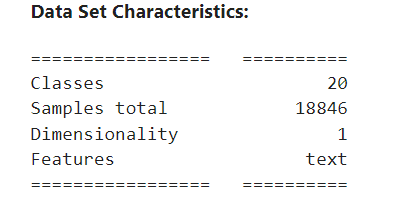
\includegraphics[width=0.45\textwidth]{imagen_1.png}  % Ajusta el nombre y la ruta de la imagen
\end{figure}

\begin{lstlisting}
# The set of targets in this dataset are the newgroup topics:
twenty_train.target_names
\end{lstlisting}

\begin{figure}[h]
    \centering
    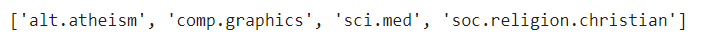
\includegraphics[width=0.8\textwidth]{imagen_2.png}  % Ajusta el nombre y la ruta de la imagen
\end{figure}

\begin{lstlisting}
# Let's examine one data point
print(twenty_train.data[3])
\end{lstlisting}

\end{frame}



\begin{frame}[fragile]{Classification Dataset: Twenty Newsgroups}

\begin{figure}[h]
    \centering
    
\includegraphics[width=0.8\textwidth]{imagen_3.png}  % Ajusta el nombre y la ruta de la imagen
\end{figure}

\begin{lstlisting}
# We have about 2k data points in total
print(len(twenty_train.data))

\end{lstlisting}

\begin{figure}[h]
    \centering
    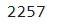
\includegraphics[width=0.09\textwidth]{imagen_4.png}  % Ajusta el nombre y la ruta de la imagen
\end{figure}
\end{frame}



\begin{frame}[fragile]{Classification Dataset: Twenty Newsgroups}
Let's see an example of Bag-of-Words on \textbf{20-newsgroups}.

\vspace{0.2cm}


We start by computing these features using the \textbf{sklearn} library.

\begin{lstlisting}
from sklearn.feature_extraction.text import CountVectorizer

# vectorize the training set
count_vect = CountVectorizer(binary=True)
X_train = count_vect.fit_transform(twenty_train.data)
X_train.shape
\end{lstlisting}

\begin{figure}[h]
    \centering
    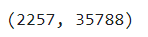
\includegraphics[width=0.21\textwidth]{imagen_5.png}  % Ajusta el nombre y la ruta de la imagen
\end{figure}

The `sklearn` count vectorizer gives us mappings between words and indices:

\begin{lstlisting}
print('Word to index `.vocabulary`: ', str(count_vect.vocabulary_)[:94] + ' ...')
feature_names = count_vect.get_feature_names_out()
print('Index to word: ', feature_names[:10])
\end{lstlisting}


\end{frame}

\begin{frame}[fragile]{Classification Dataset: Twenty Newsgroups}



\begin{figure}[h]
    \centering
    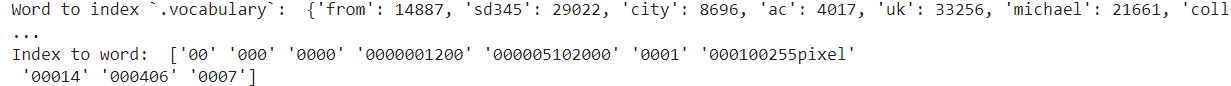
\includegraphics[width= 0.94\textwidth]{imagen_6.png}  % Ajusta el nombre y la ruta de la imagen
\end{figure}

We can retrieve the index of $\phi(x)$ associated with each `word` using these mappings:

\begin{lstlisting}
# The CountVectorizer class records the index j associated with each word in V
print('Index for the word "church": ', count_vect.vocabulary_.get(u'church'))
print('Index for the word "computer": ', count_vect.vocabulary_.get(u'computer'))

# And we can map the indices back to words
print("Word for the index '8609': ", feature_names[8609])
print("Word for the index '10000': ", feature_names[10000])
\end{lstlisting}

\begin{figure}[h]
    \centering
    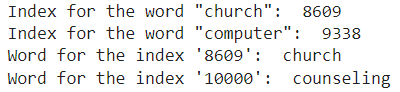
\includegraphics[width=0.4\textwidth]{imagen_7.png}  % Ajusta el nombre y la ruta de la imagen
\end{figure}


\end{frame}

\begin{frame}[fragile]{Classification Dataset: Twenty Newsgroups}

Our featurized dataset is in the matrix \texttt{X\_train}. We can use the above indices to retrieve the 0-1 value that has been computed for each word:

\begin{lstlisting}
# We can examine if any of these words are present in our previous datapoint
print(twenty_train.data[3])

# let's see if it contains these two words?
print('---'*20)
print('Value at the index for the word "church": ', X_train[3, count_vect.vocabulary_.get(u'church')])
print('Value at the index for the word "computer": ', X_train[3, count_vect.vocabulary_.get(u'computer')])
print('Value at the index for the word "doctor": ', X_train[3, count_vect.vocabulary_.get(u'doctor')])
print('Value at the index for the word "important": ', X_train[3, count_vect.vocabulary_.get(u'important')])

\end{lstlisting}
\end{frame}


\begin{frame}[fragile]{Classification Dataset: Twenty Newsgroups}



\begin{figure}[h]
    \centering
    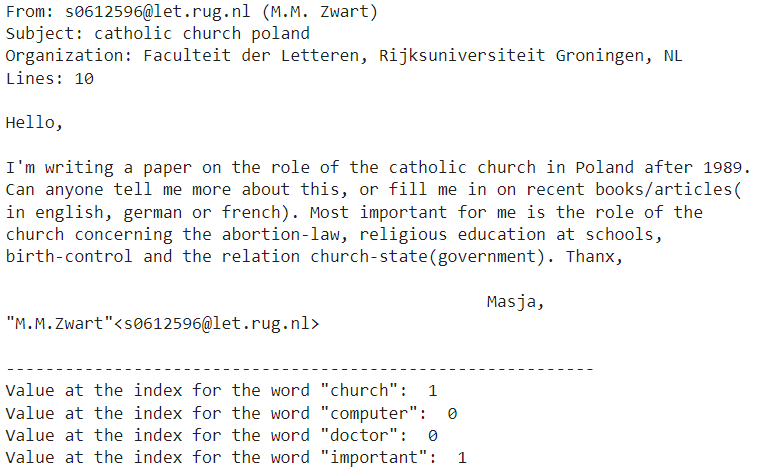
\includegraphics[width=0.7\textwidth]{imagen_8.png}  % Ajusta el nombre y la ruta de la imagen
\end{figure}
\end{frame}



\begin{frame}[fragile]{Practical Considerations}
In practice, we may use some additional modifications of this technique:


\begin{itemize}
    \item Sometimes, the feature $\phi(x)_j$ for the $j$-th word holds the count of occurrences of word $j$ instead of just the binary occurrence.
    \item The raw text is usually preprocessed. One common technique is \textit{stemming}, in which we only keep the root of the word.
    \begin{itemize}
        \item e.g. "slowly", "slowness", both map to "slow".
    \end{itemize}
    \item Filtering for common \textit{stopwords} such as "the", "a", "and". Similarly, rare words are also typically excluded.
\end{itemize}

\end{frame}

\begin{frame}[fragile]{Classification Using BoW Features}
Let's now have a look at the performance of classification over bag of words features.
\vspace{0.2cm}

Now that we have a feature representation $\phi(x)$, we can apply the classifier of our choice, such as logistic regression.



\begin{lstlisting}
from sklearn.linear_model import LogisticRegression

# Create an instance of Softmax and fit the data.
logreg = LogisticRegression(C=1e5, multi_class='multinomial', verbose=True)
logreg.fit(X_train, twenty_train.target) 
\end{lstlisting}


\end{frame}


\begin{frame}[fragile]{Classification Using BoW Features}



\begin{figure}[h]
    \centering
    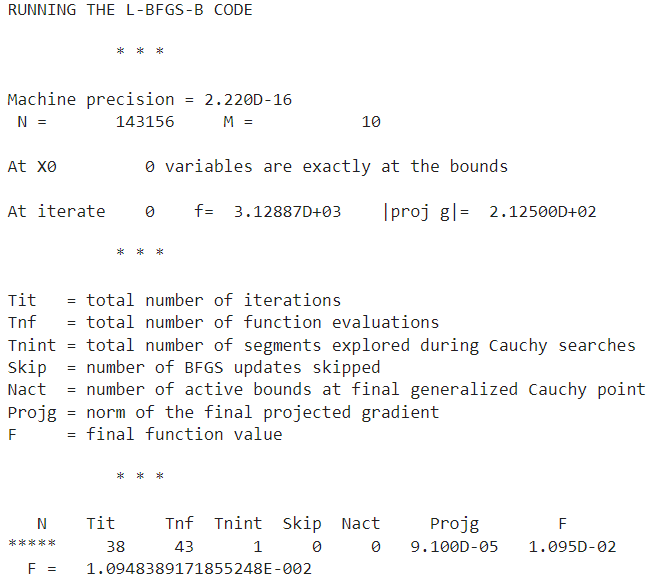
\includegraphics[width=0.7\textwidth]{imagen_9.png}  % Ajusta el nombre y la ruta de la imagen
\end{figure}


\end{frame}


\begin{frame}[fragile]{Classification Using BoW Features}

And now we can use this model for predicting on new inputs.


\begin{lstlisting}
docs_new = ['God is love', 'OpenGL on the GPU is fast']

X_new = count_vect.transform(docs_new)
predicted = logreg.predict(X_new)

for doc, category in zip(docs_new, predicted):
    print('%r => %s' % (doc, twenty_train.target_names[category]))
\end{lstlisting}

\begin{figure}[h]
    \centering
    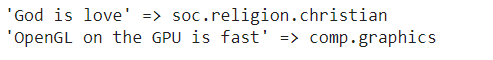
\includegraphics[width=0.5\textwidth]{imagen_10.png}  % Ajusta el nombre y la ruta de la imagen
\end{figure}

\end{frame}

\begin{frame}[fragile]{Generative Classifers for Text}

In this lecture, we are going to look at generative classifiers and their applications to text classification.
\vspace{0.2cm}


\textbf{Review: Supervised Learning Models
}
A supervised learning model can be seen as directly predicting a one-hot embedding of the target class:

$$
\underbrace{\left[ 
\begin{array}{c}
x_1 \\
x_2 \\
x_3 \\
x_4 \\
\end{array}
\right]}_\text{input}
{\to}\text{model $f_\theta(x)$}{\to}
\underbrace{\left[ 
\begin{array}{c}
0 \\
1 \\
0 \\
\end{array}
\right]}_\text{output}
$$

In this example, the $f_\theta(x)$ predicts the second class for input $x$.


\end{frame}


\begin{frame}[fragile]{Generative Classifers for Text}



\textbf{Review: Probabilistic Models
}
A probabilistic model outputs a vector of class probabilities

$$
\underbrace{\left[ 
\begin{array}{c}
x_1 \\
x_2 \\
x_3 \\
x_4 \\
\end{array}
\right]}_\text{input}
{\to}\text{model $P_\theta(y|x)$}{\to}
\underbrace{\left[ 
\begin{array}{c}
0.1 \\
0.7 \\
0.2 \\
\end{array}
\right]}_\text{output}
$$

Here, the $P_\theta(y|x)$ still predicts the second class for input $x$.

\end{frame}



\begin{frame}[fragile]{Generative Classifers for Text}


\textbf{Review: Logistic Regression
}
For example, a logistic (softmax) model outputs a probability distribution 

$$
P_\theta(y| x) 
= \left[ \begin{array}{c}
P_\theta(y=0| x) \\
P_\theta(y=1| x) \\
\end{array} \right]
= \left[ \begin{array}{c}
1-\sigma(\theta^\top x) \\
\sigma(\theta^\top x) \\
\end{array} \right]
$$

where $\theta^\top x$ is a linear model and
$$\sigma(z) = \frac{1}{1 + \exp(-z)}$$
is the \textit{sigmoid} or \textit{logistic} function.


\end{frame}


\begin{frame}[fragile]{Discriminative vs. Generative Classifers}


Logistic regression is an example of a \textit{discriminative} machine learning classifier.
$$
P_\theta(y| x) 
= \left[ \begin{array}{c}
P_\theta(y=0| x) \\
P_\theta(y=1| x) \\
\end{array} \right]
$$
\begin{itemize}
    \item It directly transforms $x$ into a score for each class $y$ (e.g., via the formula $\sigma(\theta^\top x)$)
    \item It can be interpreted as defining a \textit{conditional} probability $P_\theta(y|x)$
\end{itemize}

\end{frame}





\begin{frame}[fragile]{Example: Gaussian Discriminant Analysis}

Suppose we want to train a classifier over Iris flowers. In GDA, we define \textbf{Gaussian} probabilities:
\begin{align*}
P_\theta(x|y=\text{setosa}) && P_\theta(x|y=\text{non-setosa})
\end{align*}

as well as prior probabilities $P_\theta(y=\text{setosa}), P_\theta(y=\text{non-setosa})$.


\vspace{0.2cm}

Each Gaussian $P_\theta(x|y=\text{setosa/non-setosa})$ matches the mean and variance of the class. The $P(y)$ measures the frequency of each class $y$.

\end{frame}


\begin{frame}[fragile]{Predictions From Generative Classifiers}


Given a new $x'$, we would compare the probabilities of both models:

\begin{align*}
P_\theta(x'|y=\text{0})P_\theta(y=\text{0}) && \text{vs.} && P_\theta(x'|y=\text{1})P_\theta(y=\text{1})
\end{align*}

We output the class that's more likely to have generated $x'$.


Formally, given a new $x'$, we return the most likely class to have generated it:

\begin{align*}
\arg \max_k P_\theta(y=k | x') & = \arg \max_k  \frac{P_\theta(x' | y=k) P_\theta(y=k)}{P_\theta(x')} \\
& = \arg \max_k P_\theta(x' | y=k) P_\theta(y=k),
\end{align*}

where we have applied Bayes' rule in the first line.

\end{frame}

\begin{frame}[fragile]{A Generative Model for Text Classification}


In binary text classification, we fit two models on a labeled corpus:
\begin{align*}
P_\theta(x|y=\text{0}) && \text{and} && P_\theta(x|y=\text{1})
\end{align*}


Each model $P_\theta(x | y=k)$ \textit{scores} \textit{x} based on how much it looks like class \textit{k}.
The documents \textit{x} are in \textbf{bag-of-words} representation.

\vspace{0.2cm}

How do we choose $P_\theta(x|y=k)$?
\end{frame}

\begin{frame}[fragile]{Review: Categorical Distribution}


A Categorical distribution with parameters $\theta$ is a probability
over $K$ discrete outcomes $x \in \{1,2,...,K\}$:

$$
P_\theta(x = j) = \theta_j.
$$

When $K=2$ this is called the Bernoulli.



\end{frame}

\begin{frame}[fragile]{First Attempt at a Generative Model}

A first solution is to assume that $P(x|y=\text{spam})$ is a categorical distribution that assigns a probability to each possible word $x'=[0,1,0,...,0]$:
$$
P(x=x'|y=\text{spam}) = P \left( 
\begin{array}{c}
0 \\
1 \\
0 \\
\vdots \\
0 
\end{array}
\right.
\left.
\begin{array}{l}
\;\text{church} \\
\;\text{doctor} \\
\;\text{fervently} \\
\vdots \\
\;\text{purple}
\end{array}
\right) = \theta_{x'} = 0.0012
$$
The $\theta_{x'}$ is the probability of $x'$ under class $\text{spam}$. 
We need to specify $\theta_{x}$ for all $x$.


\end{frame}

\begin{frame}[fragile]{The Naive Bayes Assumption }

The Naive Bayes assumption is a \textbf{general technique} that can be used with any $d$-dimensional $x$ to construct tractable models $P_\theta(x|y)$ as follows:

$$
 P_{\theta} \left( x=
\begin{array}{c}
0 \\
1 \\
0 \\
\vdots \\
0 
\end{array}
\right.
\left.
\begin{array}{l}
\;\text{church} \\
\;\text{doctor} \\
\;\text{fervently} \\
\vdots \\
\;\text{purple}
\end{array}
\right) = P_\theta(x_1=0) \cdot P_\theta(x_2=1) \cdot ... \cdot P_\theta(x_d=0)
$$

Each $P_\theta(x_j=0)$ is a Bernoulli. 

\end{frame}

\begin{frame}[fragile]{The Naive Bayes Assumption }


How many parameters do we need to specify this probability?

$$
 P_{\theta} \left( x=
\begin{array}{c}
0 \\
1 \\
0 \\
\vdots \\
0 
\end{array}
\right.
\left.
\begin{array}{l}
\;\text{church} \\
\;\text{doctor} \\
\;\text{fervently} \\
\vdots \\
\;\text{purple}
\end{array}
\right) = P_\theta(x_1=0) \cdot P_\theta(x_2=1) \cdot ... \cdot P_\theta(x_d=0)
$$

This typically makes the number of parameters linear instead of exponential in $d$.

\vspace{0.2cm}

Formally, the Naive Bayes assumptions is defined as follows:

 \begin{itemize}
     \item We define the probability that $x$ takes value $x'$ to be a product of independent terms (one for each attribute $x_j$): $$ P_\theta(x=x'|y) = \prod_{j=1}^d P_\theta(x_j = x_j' \mid y) $$
     \item Each $P_\theta(x_j = x_j' \mid y)$ is typically defined to be a simple distribution like a Bernoulli.
 \end{itemize}


\end{frame}

\begin{frame}[fragile]{Naive Bayes Assumption for Bag of Words}

To deal with high-dimensional $x$, we choose a simpler model for $P_\theta(x|y)$:
\vspace{0.2cm}

1. We define the model $P_\theta(x|y=k)$ for documents $x$ as the product of the occurrence probabilities of each of its words $x_j$:
    $$ P_\theta(x = x'|y=k) = \prod_{j=1}^d P_\theta(x_j = x_j' \mid y=k) $$

2. We define a (Bernoulli) model with one parameter $\psi_{jk} \in [0,1]$ for the occurrence of each word $j$ in class $k$:
    $$P_\theta(x_j = 1 \mid y=k) = \psi_{jk} \;\;\;\;\; P_\theta(x_j = 0 \mid y=k) = 1-\psi_{jk}$$
    $\psi_{jk}$ is the probability that a document of class $k$ contains word $j$.



\end{frame}

\begin{frame}[fragile]{Naive Bayes Assumption for Bag of Words}

How many parameters does this new model have?

\begin{itemize}
    \item We have $K$ distributions of the form $P_\theta(x|y=k)$.
    \item The distribution $P_\theta(x|y=k) = \prod_{j=1}^d P_\theta(x_j \mid y=k)$ is the product of $d$ such one-parameter distributions.
    \item We have a distribution $P_\theta(x_j = 1 \mid y=k)$ for each word $j$ and each distribution has one parameter $\psi_{jk}$.
\end{itemize}

Thus, we only need $Kd$ parameters instead of $K(2^d-1)$!

\end{frame}

\begin{frame}[fragile]{Is Naive Bayes a Good Assumption?}



Naive Bayes assumes that words are uncorrelated, but in reality they are.
  \begin{itemize}
      \item If spam email contains "bank", it probably contains "account"
  \end{itemize}

As a result, the probabilities estimated by Naive Bayes can be over- under under-confident.

\vspace{0.2cm}

In practice, however, Naive Bayes is a very useful assumption that gives very good classification accuracy!



\end{frame}
\begin{frame}[fragile]{Defining Prior Distributions }


A full generative model still requires defining the distribution $P_\theta(y=k)$.

\begin{itemize}
    \item This encodes our prior belief about $y$ before we see $x$.
    \item It can also be learned from data.
\end{itemize}

\vspace{0.2cm}


Since we have a small number of classes $K$, we may use a Categorical distribution with parameters $\vec\phi = (\phi_1,...,\phi_K)$ and learn $\vec\phi$ from data:

$$ P_\theta(y=k) = \phi_k.$$

\end{frame}

\begin{frame}[fragile]{Bernoulli Naive Bayes Model}



The \textit{Bernoulli Naive Bayes} model $P_\theta(x,y)$ is defined for \textit{binary data} $x \in \{0,1\}^d$ (e.g., bag-of-words documents).

\vspace{0.2cm}


The $\theta$ contains prior parameters $\vec\phi = (\phi_1,...,\phi_K)$ and $K$ sets of per-class parameters $\psi_k = (\psi_{1k},...,\psi_{dk})$.

\vspace{0.2cm}

\begin{itemize}
    \item The probability of the data $x$ for each class equals
\end{itemize}
$$P_\theta(x|y=k) = \prod_{j=1}^d P(x_j \mid y=k),$$
where each $P_\theta(x_j \mid y=k)$ is a $\text{Bernoulli}(\psi_{jk})$.

\vspace{0.2cm}

\begin{itemize}
    \item The probability over $y$ is Categorical: $P_\theta(y=k) = \phi_k$.
\end{itemize}

\end{frame}

\begin{frame}[fragile]{Bernoulli Naive Bayes Model}

Formally, we have:
\begin{align*}
P_\theta(y) & = \text{Categorical}(\phi_1,\phi_2,\ldots,\phi_K) \\
P_\theta(x_j=1|y=k) & = \text{Bernoulli}(\psi_{jk}) \\
P_\theta(x|y=k) & = \prod_{j=1}^d P_\theta(x_j|y=k)
\end{align*}
The parameters of the model are $\theta = (\phi_1,...,\phi_K, \psi_{11}, ...,\psi_{dK})$.
There are exactly $K(d+1)$ parameters.
\end{frame}


\begin{frame}[fragile]{The Parameters of a Naive Bayes Model}

We need to learn the parameters of two sets of distributions:
 \begin{itemize}
     \item The distribution over classes is Categorical, denoted $\text{Categorical}(\phi_1, \phi_2, ..., \phi_K)$. Thus, $P_\theta(y=k) = \phi_k$.
     \item The conditional probability $P(x\mid y=k)$ of the data under class $k$ is a product of Bernoullis $$P_\theta(x|y=k) = \prod_{j=1}^d P(x_j \mid y=k),$$ where each $P_\theta(x_j \mid y=k)$ is a $\text{Bernoulli}(\psi_{jk})$.
 \end{itemize}
\end{frame}


\begin{frame}[fragile]{Learning the Parameters $\phi$}


Consider learning $\vec \phi = (\phi_1, \phi_2, \ldots, \phi_K)$. 

\begin{itemize}
    \item We have $n$ datapoints. Each point has a label $k\in\{1,2,...,K\}$.
    \item Our model is a categorical and assigns a probability $\phi_k$ to each outcome $k\in\{1,2,...,K\}$.
    \item We want to infer $\phi_k$ assuming our dataset is sampled from the model.
\end{itemize}

What are the maximum likelihood $\phi_k$ that are most likely to have generated our data?

\vspace{0.2cm}

Intuitively, the class probabilities $\phi$ should just be the class proportions that we see in the data. 
$$ \phi_k = \frac{n_k}{n}$$
for each $k$, where $n_k = |\{i : y^{(i)} = k\}|$ is the number of training targets with class $k$.

Thus, the optimal $\phi_k$ is just the proportion of data points with class $k$ in the training set!
\end{frame}

\begin{frame}[fragile]{Learning the Parameters $\psi_{jk}$}

Next we want to learn the parameter $\psi_{jk}$ (i.e., probability that $x_j=1$ given class $k$).

 \begin{itemize}
     \item For each $k$, consider all the inputs $x$ for which $y=k$.
     \item We seek  the probability $\psi_{jk}$ of a word $j$ being present in an $x$.
 \end{itemize}


What is the optimal $\psi_{jk}$ in this case?

\vspace{0.2cm}

Each $\psi_{jk}$ is simply the proportion of documents in class $k$ that contain the word $j$.
\begin{align*}
\psi_{jk} = \frac{n_{jk}}{n_k}.
\end{align*}
where $|\{i : x^{(i)}_j = 1 \text{ and } y^{(i)} = k\}|$ is the number of $x^{(i)}$ with label $k$ and a positive occurrence of word $j$.

\end{frame}

\begin{frame}[fragile]{Querying the Model}



How do we ask the model for predictions? As discussed earlier, we can apply Bayes' rule:
$$\arg\max_y P_\theta(y|x) = \arg\max_y P_\theta(x|y)P(y).$$
Thus, we can estimate the probability of $x$ and under each $P_\theta(x|y=k)P(y=k)$ and choose the class that explains the data best.

\vspace{0.2cm}

\textbf{Classification Dataset: Twenty Newsgroups}

To illustrate the text classification problem, we will use a popular dataset called \textbf{20-newsgroups}. 


\begin{itemize}
    \item It contains ~20,000 documents collected approximately evenly from 20 different online newsgroups.
    \item Each newgroup covers a different topic such as medicine, computer graphics, or religion.
    \item This dataset is widely used to benchmark text classification and other types of algorithms.
\end{itemize}

\end{frame}

\begin{frame}[fragile]{Classification Dataset: Twenty Newsgroups}

Let's load this dataset.


\begin{lstlisting}
#https://scikit-learn.org/stable/tutorial/text_analytics/working_with_text_data.html
from sklearn.datasets import fetch_20newsgroups

# for this lecture, we will restrict our attention to just 4 different newsgroups:
categories = ['alt.atheism', 'soc.religion.christian', 'comp.graphics', 'sci.med']
twenty_train = fetch_20newsgroups(subset='train', categories=categories, shuffle=True, random_state=42)
Markdown(twenty_train.DESCR[:1088]);
\end{lstlisting}
\end{frame}

\begin{frame}[fragile]{Example: Text Classification}

Let's see how this approach can be used in practice on the text classification dataset.
 \begin{itemize}
     \item We will learn a good set of parameters for a Bernoulli Naive Bayes model
     \item We will compare the outputs to the true predictions.
 \end{itemize}

Let's see an example of Naive Bayes on \texttt{20-newsgroups}.

We start by computing these features using the \texttt{sklearn} library.


\begin{lstlisting}
from sklearn.feature_extraction.text import CountVectorizer

# vectorize the training set
count_vect = CountVectorizer(binary=True, max_features=1000)
y_train = twenty_train.target
X_train = count_vect.fit_transform(twenty_train.data).toarray()
feature_names = count_vect.get_feature_names_out()
X_train.shape

\end{lstlisting}

\begin{figure}[h]
    \centering
    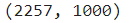
\includegraphics[width=0.2\textwidth]{pic1.png}  % Ajusta el nombre y la ruta de la imagen
\end{figure}
\end{frame}

\begin{frame}[fragile]{Example: Text Classification}

Let's compute the maximum likelihood model parameters on our dataset. This is done in closed-form by just estimating statistics on the data, so we don't need to do gradient descent.


\begin{lstlisting}
n = X_train.shape[0] # size of the dataset
d = X_train.shape[1] # number of features in our dataset
K = 4 # number of clases

# these are the shapes of the parameters
psis = np.zeros([K,d])
phis = np.zeros([K])
# we now compute the parameters
for k in range(K):
    X_k = X_train[y_train == k]
    psis[k] = np.mean(X_k, axis=0)
    phis[k] = X_k.shape[0] / float(n)
# print out the class proportions
print(phis)
\end{lstlisting}

\begin{figure}[h]
    \centering
    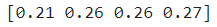
\includegraphics[width=0.33\textwidth]{pic2.png}  % Ajusta el nombre y la ruta de la imagen
\end{figure}
\end{frame}

\begin{frame}[fragile]{Example: Text Classification}

The learned parameters contain information about the \textbf{most frequent words}:

\begin{lstlisting}
top_words = []
for category in range(4):
    top_words.append(feature_names[np.argsort(psis[category])[-200:]])

for category in range(4):
    words_from_other_categories = np.concatenate(top_words[:category] + top_words[category+1:])
    unique_words = [word for word in top_words[category] if word not in words_from_other_categories]
    print(f'\n# top 10 ~unique words occurring in {twenty_train.target_names[category]}:')
    print(unique_words[-10:])
\end{lstlisting}

\begin{figure}[h]
    \centering
    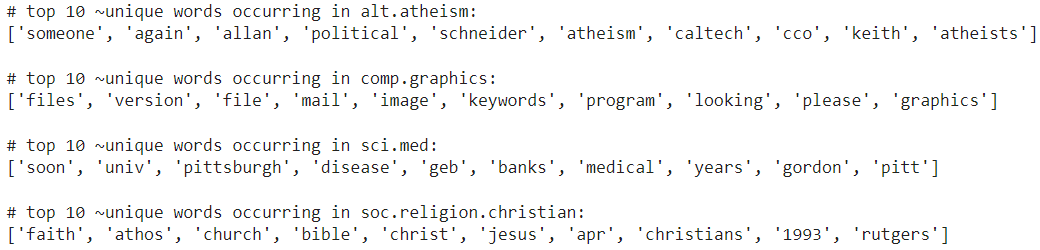
\includegraphics[width=0.65\textwidth]{pic3.png}  % Ajusta el nombre y la ruta de la imagen
\end{figure}
\end{frame}
\begin{frame}[fragile]{Example: Text Classification}

We can compute \textbf{predictions} using Bayes' rule.


\begin{lstlisting}
def nb_predictions(x, psis, phis):
    """This returns class assignments and scores under the NB model.
    
    We compute \arg\max_y p(y|x) as \arg\max_y p(x|y)p(y)
    """
    # adjust shapes
    n, d = x.shape
    x = np.reshape(x, (1, n, d))
    psis = np.reshape(psis, (K, 1, d))
    
    psis = psis.clip(1e-14, 1-1e-14) # clip probabilities to avoid log(0)
    
    # compute log-probabilities
    logpy = np.log(phis).reshape([K,1])
    logpxy = x * np.log(psis) + (1-x) * np.log(1-psis)
    logpyx = logpxy.sum(axis=2) + logpy


\end{lstlisting}
\end{frame}

\begin{frame}[fragile]{Example: Text Classification}
\begin{lstlisting}[firstnumber=17]
    return logpyx.argmax(axis=0).flatten(), logpyx.reshape([K,n])
    
idx_train, logpyx = nb_predictions(X_train, psis, phis)
print(idx_train[:10])
\end{lstlisting}

\begin{figure}[h]
    \centering
    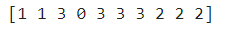
\includegraphics[width=0.3\textwidth]{pic4.png}  % Ajusta el nombre y la ruta de la imagen
\end{figure}

We can measure the \textbf{accuracy}:

\begin{lstlisting}
(idx_train==y_train).mean()
\end{lstlisting}

\begin{figure}[h]
    \centering
    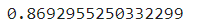
\includegraphics[width=0.3\textwidth]{pic5.png}  % Ajusta el nombre y la ruta de la imagen
\end{figure}
\end{frame}

\begin{frame}[fragile]{Example: Text Classification}

We can also \textbf{make up new queries} and \textbf{ask the model} to label them:

\begin{lstlisting}
docs_new = ['OpenGL on the GPU is fast']

X_new = count_vect.transform(docs_new).toarray()
predicted, logpyx_new = nb_predictions(X_new, psis, phis)

for doc, category in zip(docs_new, predicted):
    print('%r => %s' % (doc, twenty_train.target_names[category]))
\end{lstlisting}

\begin{figure}[h]
    \centering
    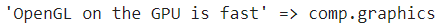
\includegraphics[width=0.55\textwidth]{pic6.png}  % Ajusta el nombre y la ruta de la imagen
\end{figure}




\end{frame}
\end{document}
